\documentclass[12pt, a4paper]{article}
\usepackage[top=3cm, bottom=4cm, left=3.5cm, right=3.5cm]{geometry}
\usepackage{amsmath,amsthm,amsfonts,amssymb,amscd, fancyhdr, color, comment, graphicx, environ}
\usepackage{float}
\usepackage{mathrsfs}
\usepackage{lastpage}
\usepackage[dvipsnames]{xcolor}
\usepackage[framemethod=TikZ]{mdframed}
\usepackage{enumerate}
\usepackage[shortlabels]{enumitem}
\usepackage{fancyhdr}
\usepackage{indentfirst}
\usepackage{listings}
\usepackage{sectsty}
\usepackage{thmtools}
\usepackage{shadethm}
\usepackage{hyperref}
\usepackage{setspace}
\usepackage{enumitem}
\usepackage{systeme} 
\usepackage[portuguese]{babel}
\selectlanguage{portuguese}
\hypersetup{
    colorlinks=true,
    linkcolor=blue,
    filecolor=magenta,      
    urlcolor=blue,
}
%%%%%%%%%%%%%%%%%%%%%%%%%%%%%%%%%%%%%%%%%%%%%%%%%%%%%%%%%%%%%%%%%%
%%%%%%%%%%%%%%%%%%%%%%%%%%%%%%%%%%%%%%%%%%%%%%%%%%%%%%%%%%%%%%%%%%

\mdtheorem[style=theoremstyle]{Problem}{Problem}
\newenvironment{Solution}{\textbf{Solution.}}

%%%%%%%%%%%%%%%%%%%%%%%%%%%%%%%%%%%%%%%%%%%%%%%%%%%%%%%%%%%%%%
%Page setup
\pagestyle{fancy}
\headheight 35pt
\rhead{
\includegraphics[width=2.5cm]{2_49.png}} %
\lfoot{}
\lhead{}
\pagenumbering{arabic}
\cfoot{\small\thepage}
\rfoot{}
\headsep 1.2em
\renewcommand{\baselinestretch}{1.25}       
\mdfdefinestyle{theoremstyle}{%
linecolor=black,linewidth=1pt,%
frametitlerule=true,%
frametitlebackgroundcolor=gray!20,
innertopmargin=\topskip,
}
%%%%%%%%%%%%%%%%%%%%%%%%%%%%%%%%%%%%%%%%%%%%%%%%%%%%%%%%%%%%%%%%%%
%%%%%%%%%%%%%%%%%%%%%%%%%%%%%%%%%%%%%%%%%%%%%%%%%%%%%%%%%%%%%%%%%%
%Add new commands here
\renewcommand{\labelenumi}{\alph{enumi})}
\newcommand{\Z}{\mathbb Z}
\newcommand{\R}{\mathbb R}
\newcommand{\Q}{\mathbb Q}
\newcommand{\NN}{\mathbb N}
\DeclareMathOperator{\Mod}{Mod} 
\renewcommand\lstlistingname{Algorithm}
\renewcommand\lstlistlistingname{Algorithms}
\def\lstlistingautorefname{Alg.}
%%%%%%%%%%%%%%%%%%%%%%%%%%%%%%%%%%%%%%%%%%%%%%%%%%%%%%%%%%%%%%%%%%


\begin{document}

\begin{titlepage}
    \begin{center}
        \vspace*{3cm}
            
        \Huge
        \textbf{MAP2212}
            
        \vspace{1cm}
        \huge
        Laboratório de Computação e Simulação \\
            
        \vspace{1.5cm}
        \Large
            
        \textbf{Enzo Valentim Cappelozza \\ Lucas Panfilo Donaire}                      % <-- author
        
            
        \vfill
        
        Professor:  \\
        Julio Michael Stern
            
        \vspace{1cm}
            
        
\includegraphics[width=0.4\textwidth]{2_49.png}
        \\
        
        \Large
        
        \today
            
    \end{center}
\end{titlepage}

%%%%%%%%%%%%%%%%%%%%%%%%%%%%%%%%%%%%%%%%%%%%%%%%%%

\newpage
\section{Introdução}
O presente trabalho tem por finalidade realizar uma análise do método de \textit{Monte-Carlo Markov Chain} para a geração variáveis aleatórias com distribuição \textit{Dirichlet} no simplex $S_3 = \{(\theta_1, \theta_2, \theta_3) \in \mathbb{R}^3 : \theta_1 +  \theta_2 + \theta_3 = 1\}$.

Para tal, usaremos a teoria das \textit{Cadeias de Markov} a tempo discreto, algumas noções de variáveis aleatórias e o \textit{software} Python. 

\section{Explicação do Método}

\subsection{A Teoria}
Usaremos aqui o método heurístico descrito em (ADICIONE AQUI A REFERÊNCIA DO GILKS): $$\Sigma \propto (1-\lambda)S + \lambda D $$ onde $$S = \frac{1}{n}(X-\bar{x})(X-\bar{x})^T$$ e $D$ é uma matriz diagonal cujas entradas $d_{ii}$ são as covariâncias de cada um dos vetores linha dos pontos gerados.

Por exemplo, caso tenhamos vetores da forma $X = (u, v, w)$ e $x = (x_1 | x_2 |  x_3)^T$ onde cada $x_i$ de 1 até 3 representa um vetor linha, e $\hat{x_i}$ é a média arimética simples do vetor linha, temos $\hat{x} = (\hat{x_1}, \hat{x_2}, \hat{x_3})$ como sendo o vetor das médias ariméticas dos vetores linha, assim, definimos: $\alpha = (u - \hat{x}_1)$, $\beta = (v - \hat{x}_2)$ e $\gamma = (w - \hat{x)_3}$ de tal maneira que a matriz $S$ de covariância dinâmica é: 

$$S =  \frac{1}{3}
\begin{bmatrix}
\alpha^2 & \alpha \beta & \alpha \gamma \\
\alpha \beta &  \beta^2 & \beta \gamma \\
\alpha \gamma & \beta \gamma & \gamma ^2 \\
\end{bmatrix}
$$

Por conseguinte, dado que temos que $D$ é a matriz diagonal da variância marginal, para cada vetor linha de $x$, podemos similarmente definir:

$$D = 
\begin{bmatrix}
Var(L_1) & & \\
& Var(L_2) & \\
& & Var(L_3) \\
\end{bmatrix}
$$
Onde $L_i$ é o \textit{i-ésimo} vetor linha de $x$. 

Assim, temos que 

$$
\Sigma \propto  (1-\lambda)\frac{1}{3}
\begin{bmatrix}
\alpha^2 & \alpha \beta & \alpha \gamma \\
\alpha \beta &  \beta^2 & \beta \gamma \\
\alpha \gamma & \beta \gamma & \gamma ^2 \\
\end{bmatrix}
+ \lambda
\begin{bmatrix}
Var(L_1) & & \\
& Var(L_2) & \\
& & Var(L_3) \\
\end{bmatrix}
$$

Onde $\lambda$ é uma constante de proporcionalidade que deve ser alterada dinamicamente a fim de ajustar/limitar o domínio de onde se deseja realizar o teste de aceitação/rejeição. 













\subsection{Explicação do Algoritmo}
De maneira ordenada, temos que, para simular pontos com distribuição f, executamos os seguintes passos:
dado um ponto inicial arbitrário $t_0$
%coloque aqui abaixo o método de funcionamento do algoritmo. 

\begin{enumerate}[label=(\arabic*)]
    \item enquanto temos i pontos:
    \item achamos o possível próximo ponto, $p_{i+1} = t_i +y$, tal que $y \sim N(0,\Sigma)$
    \item calculamos $\alpha = min(1, f(t_i)/f(p_{i+1}))$
    \item geramos $u \sim U[0,1]$
    \item se $\alpha > u$, aceitamos o próximo ponto, $t_{i+1} = p_{i+1}$
    \item caso contrário, voltamos a (2)
    \item se atingimos n pontos, paramos
    \item se não, voltamos a (1)
\end{enumerate}

Esse é um método de aceitação-rejeição baseado nas cadeias de Markov. Uma observação é que não usamos $t_0$ como um ponto. Ao invés disso, 'esquentamos' a cadeia rodando 100 iterações antes de começar a gerar pontos válidos de fato. A ideia é que o ponto vai se movendo para a região onde a f.d.p é maior, ou seja, ele é mais provável de ir onde a f.d.p é maior, o que é o comportamento esperado de uma variável aleatória. 
No programa em python, ao tentar gerar $\Sigma$ de acordo com o descrito acima, encontramos problemas relacionados ao nosso domínio do simplex. Então, geramos $y = [y_1,y_2,-y_1 -y_2]$, tal que $y_1,y_2 \sim N(0, 3/10)$. Apesar disso, mesmo testando diferentes variâncias da normal, os pontos pareciam mais 'concentrados' do que na Dirichlet, como se a variância caísse ao usar o MCMC. Testamos também gerar y pela distribuição t de Student, e tivemos o mesmo problema, mesmo seguindo o algorítmo a risca


\section{Testes e dados pertinentes}
Para os coeficientes de aceitação obtivemos os seguintes dados.

\begin{center}
\begin{tabular}{|c|c|c|c|c|c|c|}
\hline
& 1k & 5k & 10k& 20k & 50k & 100k \\
\hline
$\alpha$ & 0.743& 0.78 & 0.7608 & 0.77205 & 0.77608 & 0.77075 \\
\hline
\end{tabular}
\end{center}

\subsection{Inspeção visual}
Abaixo algumas imagens retiradas diretamente do \textit{Python} utilizando o pacote \textit{matplotlib}, que ilustram a geração do simplex $S_3$ a partir do método \textit{Monte-Carlo Markov Chain}.

Note: em alguns dos \textit{plots} há um ponto vermelho. Este ponto vermelho é o ponto inicial que tomamos para o nosso algoritmo. 

\begin{figure}[H]
\centering
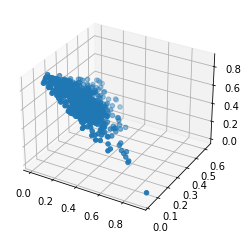
\includegraphics[scale = 0.7]{1K.png}
\includegraphics[scale = 0.7]{5K.png}
\caption{1000 e 5000 pontos, respectivamente}
\end{figure}

\begin{figure}[H]
\centering

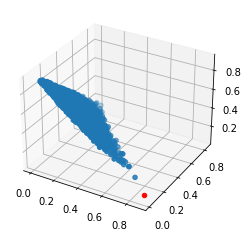
\includegraphics[scale = 0.7]{10K.png}
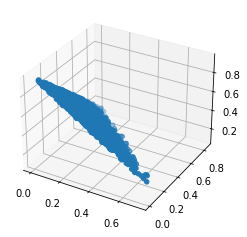
\includegraphics[scale = 0.7]{20K.png}
\caption{10.000 e 20.000 pontos, respectivamente}

\end{figure}

\begin{figure}[H]
\centering

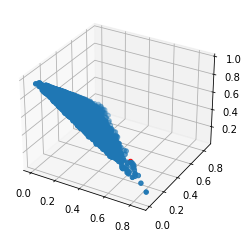
\includegraphics[scale = 0.7]{50K.png}
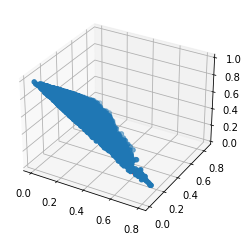
\includegraphics[scale = 0.7]{100k.png}
\caption{50.000 e 100.000 pontos, respectivamente}

\end{figure}







\end{document}


